\documentclass{article}

\usepackage[fleqn]{amsmath} % This package with the fleqn option aligns equations to the left
\setlength{\mathindent}{0pt} % Set indentation from the left margin

\usepackage{amssymb} % Required for math symbols
\usepackage{graphicx} % Required for inserting images
\usepackage{geometry}

\usepackage[section]{placeins}

\usepackage[backend=biber, style=authoryear, citestyle=authoryear]{biblatex}
\addbibresource{references.bib}

\geometry{a4paper, margin=1in}

{
\title{
    
\includegraphics[width=0.34\textwidth]{/Users/mlnick/documents/images/tsukuba-logo.png} \\
    \vspace{2mm}
    \textbf{Numerical Simulation} \\
    \vspace{3mm}    
    Hometask 3
}

\author{Mamanchuk Mykola, SID.202420671}
% \date{\today}
\date{June 14, 2024}
}

\usepackage{listings}
\usepackage{color}

\definecolor{codegreen}{rgb}{0,0.6,0}
\definecolor{codegray}{rgb}{0.5,0.5,0.5}
\definecolor{codepurple}{rgb}{0.58,0,0.82}
\definecolor{backcolour}{rgb}{0.99,0.99,0.99}

\lstdefinestyle{mystyle}{
    backgroundcolor=\color{backcolour},   
    commentstyle=\color{codegreen},
    keywordstyle=\color{magenta},
    numberstyle=\tiny\color{codegray},
    stringstyle=\color{codepurple},
    basicstyle=\ttfamily\footnotesize,
    breakatwhitespace=false,         
    breaklines=true,                 
    captionpos=b,                    
    keepspaces=true,                 
    numbers=left,                    
    numbersep=5pt,                  
    showspaces=false,                
    showstringspaces=false,
    showtabs=false,                  
    tabsize=2
}
\lstset{style=mystyle}

\begin{document}

\maketitle


\setlength{\fboxsep}{0pt} % Removes padding around the image
\setlength{\fboxrule}{0.5pt} % Sets the thickness of the border

\section{Prove Instability using Von Neumann Stability Analysis}

The task is to analyze the stability of the forward-time central-space (FTCS) scheme for the hyperbolic equation given by:
\[
\frac{u_j^{n+1} - u_j^n}{\Delta t} = -v \left(\frac{u_{j+1}^n - u_{j-1}^n}{2\Delta x}\right)
\]
using Von Neumann Stability Analysis. We are to demonstrate that this scheme is unstable.

\subsection{Analysis}

Using the Von Neumann stability analysis, we introduce the ansatz:
\[
u_j^n = \xi^n e^{ikj\Delta x}
\]
Substituting into the discretized equation and simplifying, we get:
\[
\xi^{n+1} = \xi^n \left[ 1 - i \frac{v\Delta t}{\Delta x} \sin(k\Delta x) \right]
\]
This yields the amplification factor \( \xi \) as:
\[
\xi(k) = 1 - i \frac{v\Delta t}{\Delta x} \sin(k\Delta x)
\]
To assess stability, we need \( |\xi| \leq 1 \). Calculating \( |\xi| \), we find:
\[
|\xi| = \sqrt{1 + \left(\frac{v\Delta t}{\Delta x} \sin(k\Delta x)\right)^2}
\]
Since \( \sin^2(k\Delta x) \leq 1 \), it follows that \( |\xi| \geq 1 \) for all \( k \), except possibly at \( k = 0 \). This proves that the solution is unstable as \( |\xi| > 1 \) for all \( -\pi/\Delta x < k < \pi/\Delta x \) except for \( k = 0 \).

\subsection{Solution Figures}

\textbf{During the class} I have solved this task as it is shown on the figures 1 and 2.

\begin{figure}[h!]
    \centering
    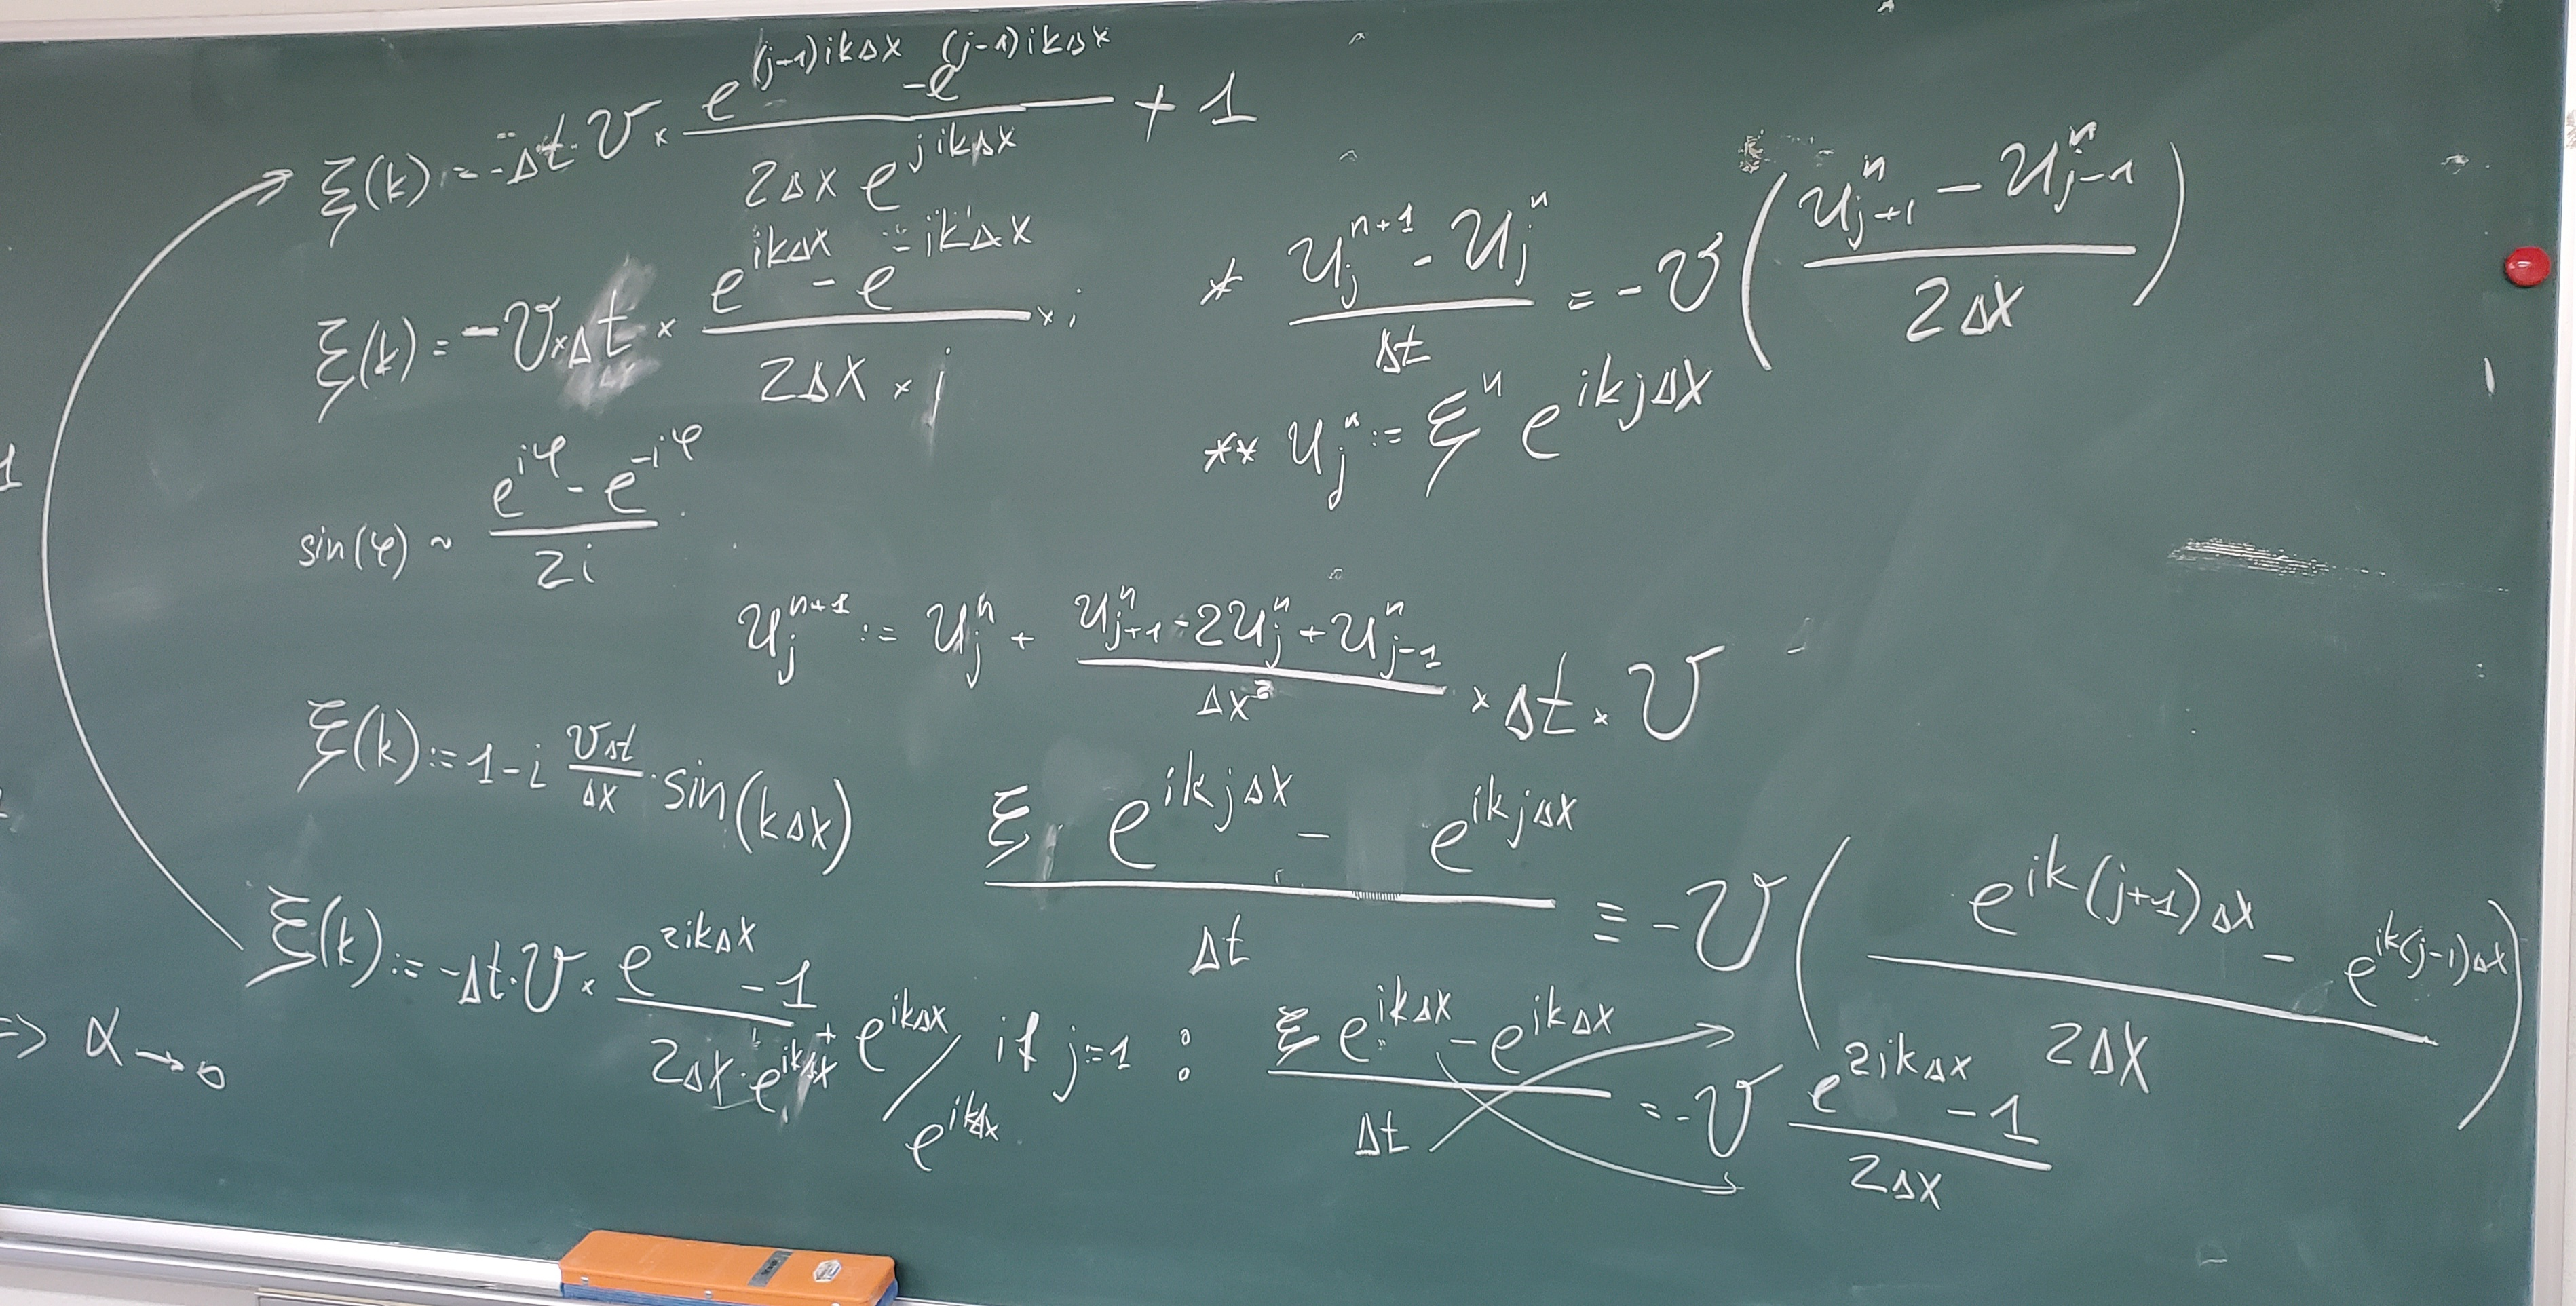
\includegraphics[width=0.8\textwidth]{materials/ph1.jpg}
    \caption{Initial part of the solution derivation.}
    \label{fig:ph1}
\end{figure}

\begin{figure} [h!]
    \centering
    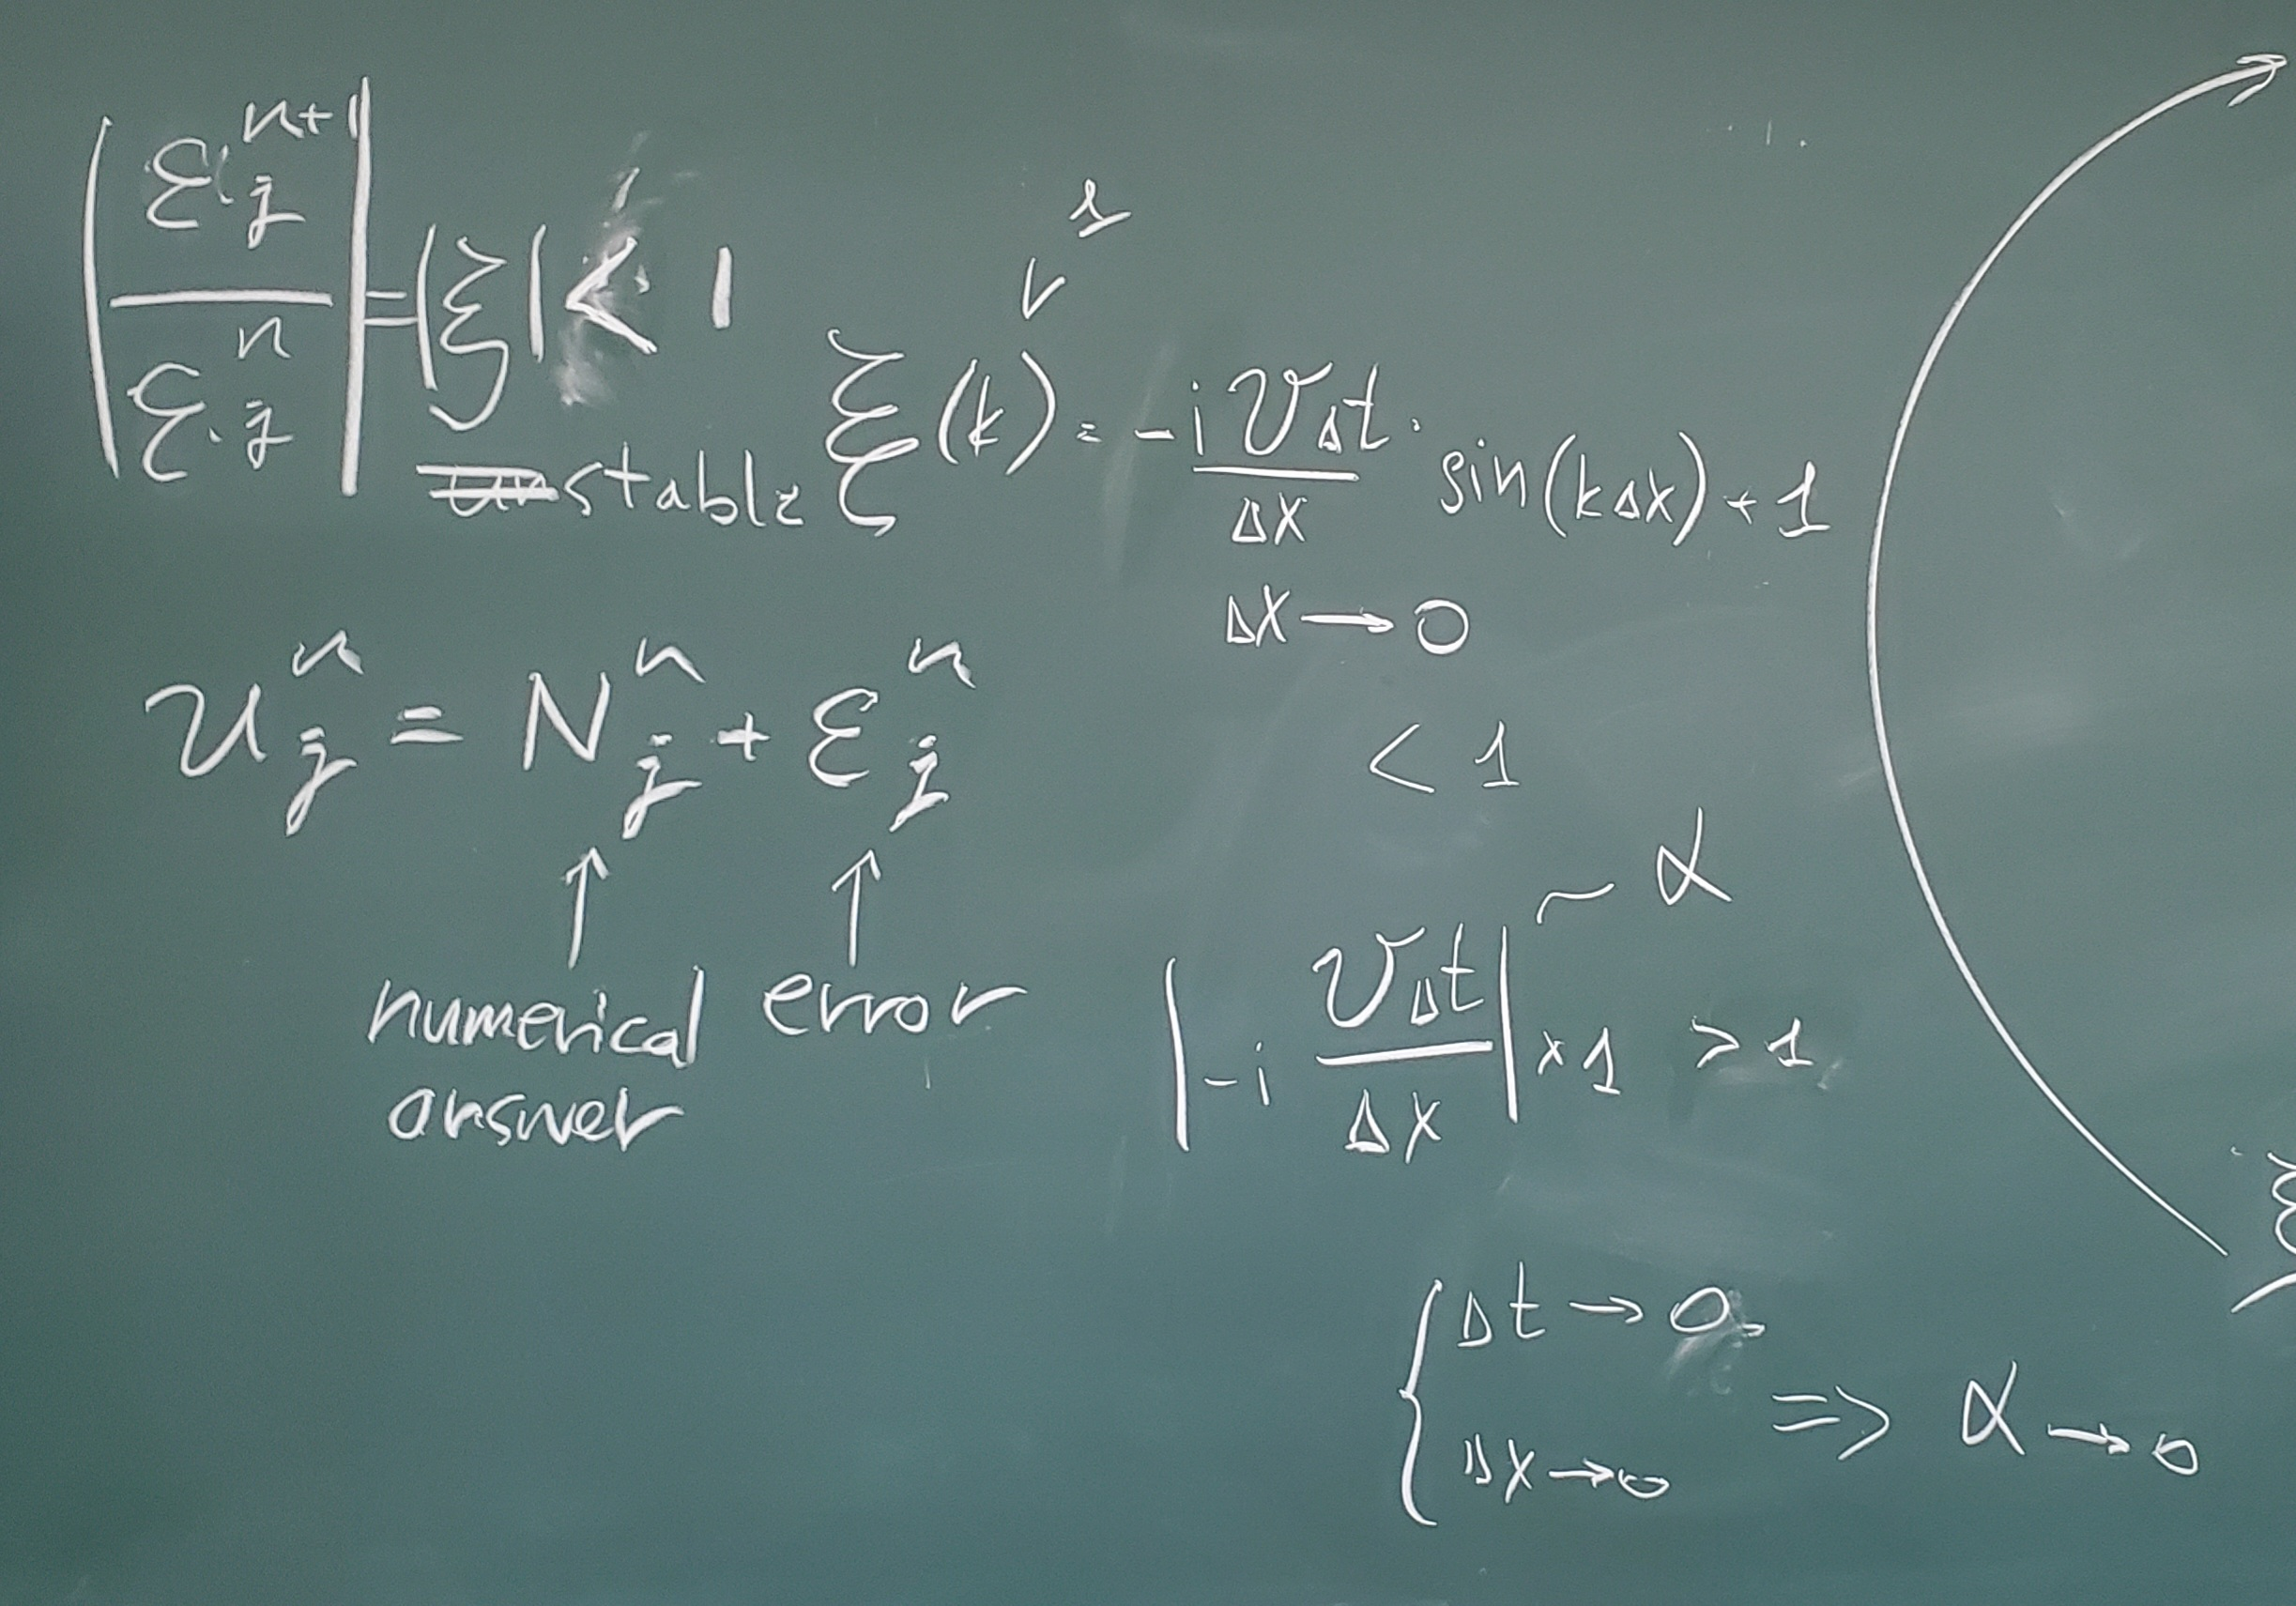
\includegraphics[width=0.6\textwidth]{materials/ph2.jpg}
    \caption{Completion of the solution derivation showing the amplification factor calculation.}
    \label{fig:ph2}
\end{figure}

\subsection{Detailed Solution}
We consider the forward-time central-space (FTCS) approximation for the hyperbolic equation:
\[
\frac{u_j^{n+1} - u_j^n}{\Delta t} = -v \left(\frac{u_{j+1}^n - u_{j-1}^n}{2\Delta x}\right)
\]
This equation can be rearranged to express the future time step \( u_j^{n+1} \) as:
\[
u_j^{n+1} = u_j^n - \frac{v\Delta t}{2\Delta x} \left(u_{j+1}^n - u_{j-1}^n\right)
\]

To apply the Von Neumann stability analysis, we introduce the ansatz:
\[
u_j^n = \xi^n e^{ikj\Delta x}
\]
Substituting this ansatz into the rearranged equation gives:
\[
\xi^{n+1} e^{ikj\Delta x} = \xi^n e^{ikj\Delta x} - \frac{v\Delta t}{2\Delta x} \left(\xi^n e^{ik(j+1)\Delta x} - \xi^n e^{ik(j-1)\Delta x}\right)
\]
This can be simplified by dividing through by \( \xi^n e^{ikj\Delta x} \), resulting in:
\[
\xi = 1 - \frac{v\Delta t}{2\Delta x} \left(e^{ik\Delta x} - e^{-ik\Delta x}\right)
\]
Using the identity for the difference of complex exponentials, \( e^{ix} - e^{-ix} = 2i\sin(x) \), we rewrite:
\[
\xi = 1 - i \frac{v\Delta t}{\Delta x} \sin(k\Delta x)
\]
The amplification factor \( \xi \) is thus given by:
\[
\xi = 1 - i \frac{v\Delta t}{\Delta x} \sin(k\Delta x)
\]
To check for stability, we calculate \( |\xi| \), the magnitude of the amplification factor:
\[
|\xi| = \sqrt{1 + \left(\frac{v\Delta t}{\Delta x} \sin(k\Delta x)\right)^2}
\]
Since \( \sin^2(k\Delta x) \leq 1 \), it follows that:
\[
|\xi| \geq 1
\]
This result implies \( |\xi| > 1 \) for any non-zero \( k\Delta x \), indicating that the scheme is unstable as the error grows exponentially with each time step. The only exception occurs at \( k = 0 \), where \( \xi = 1 \) and the scheme does not amplify errors, but this is a trivial case that does not affect the overall instability conclusion.


\section{Stability Analysis of the Diffusion Equation}
This section provides a comprehensive analysis of the stability of the numerical scheme used to approximate the diffusion equation. We employ the forward-time centered-space (FTCS) discretization and the Von Neumann stability criterion to evaluate the stability of the scheme.

\subsection{Theoretical Background}
The diffusion equation, when discretized using the FTCS approach, is represented as:
\[
\frac{u_j^{n+1} - u_j^n}{\Delta t} = D \left(\frac{u_{j+1}^n - 2u_j^n + u_{j-1}^n}{\Delta x^2}\right)
\]
This formulation leads to the update equation:
\[
u_j^{n+1} = u_j^n + \frac{D\Delta t}{\Delta x^2} (u_{j+1}^n - 2u_j^n + u_{j-1}^n)
\]

\subsection{Von Neumann Stability Analysis}
Introducing the Fourier series ansatz for \( u_j^n \):
\[
u_j^n = \xi^n e^{ikj\Delta x}
\]
where \( \xi \) is the growth factor per time step, and substituting it into the update equation, we derive:
\[
\xi^{n+1} e^{ikj\Delta x} = \xi^n e^{ikj\Delta x} + \frac{D\Delta t}{\Delta x^2} \left(\xi^n e^{ik(j+1)\Delta x} - 2\xi^n e^{ikj\Delta x} + \xi^n e^{ik(j-1)\Delta x}\right)
\]
which simplifies to:
\[
\xi = 1 + \frac{D\Delta t}{\Delta x^2} \left(e^{ik\Delta x} + e^{-ik\Delta x} - 2\right)
\]
Using the identity for the sum of exponentials, \( e^{ix} + e^{-ix} = 2\cos(x) \):
\[
\xi = 1 + \frac{2D\Delta t}{\Delta x^2} (\cos(k\Delta x) - 1)
\]
and by substituting \( \cos(k\Delta x) = 1 - 2\sin^2\left(\frac{k\Delta x}{2}\right) \):
\[
\xi = 1 - \frac{4D\Delta t}{\Delta x^2} \sin^2\left(\frac{k\Delta x}{2}\right)
\]

\subsection{Stability Condition}
For the scheme to be stable, the magnitude of \( \xi \), \( |\xi| \), must be less than or equal to 1:
\[
|\xi| = \left| 1 - \frac{4D\Delta t}{\Delta x^2} \sin^2\left(\frac{k\Delta x}{2}\right) \right| \leq 1
\]
The critical condition for stability occurs at the maximum of \( \sin^2\left(\frac{k\Delta x}{2}\right) = 1 \):
\[
\frac{4D\Delta t}{\Delta x^2} \leq 2
\]
\[
\Delta t \leq \frac{\Delta x^2}{2D}
\]

\subsection{Conclusion}
The maximum permissible time step for the stability of the FTCS scheme in simulating the diffusion equation is therefore:
\[
\Delta t \leq \frac{\Delta x^2}{2D}
\]
This condition ensures the numerical scheme remains stable without amplifying errors exponentially over time.

\section*{References}
\begin{enumerate}
    \item \textbf{Mamanchuk N., University of Tsukuba}, Github, June 14, 2024. Available online: \url{https://github.com/RIFLE}
    % \item \textbf{Company}, Name of Work, year. Available online: \url{https://...} [Accessed: yyyy-mm-dd]
\end{enumerate}

\end{document}
